%%%%%%%%%%%%%%%%%%%%%%%%%%%%%%%%%%%%%%%%%
% Short Sectioned Assignment
% LaTeX Template
% Version 1.0 (5/5/12)
%
% This template has been downloaded from:
% http://www.LaTeXTemplates.com
%
% Original author:
% Frits Wenneker (http://www.howtotex.com)
%
% License:
% CC BY-NC-SA 3.0 (http://creativecommons.org/licenses/by-nc-sa/3.0/)
%
%%%%%%%%%%%%%%%%%%%%%%%%%%%%%%%%%%%%%%%%%

%----------------------------------------------------------------------------------------
%	PACKAGES AND OTHER DOCUMENT CONFIGURATIONS
%----------------------------------------------------------------------------------------

\documentclass[paper=a4, fontsize=11pt]{scrartcl} % A4 paper and 11pt font size

\usepackage[T1]{fontenc} % Use 8-bit encoding that has 256 glyphs
%\usepackage{fourier} % Use the Adobe Utopia font for the document - comment this line to return to the LaTeX default
\usepackage[english]{babel} % English language/hyphenation
\usepackage{amsmath,amsfonts,amsthm} % Math packages
\usepackage{mathtools} %More math! (For dscases)
\usepackage{hyperref} %HTML package
\usepackage{pgfplots} %Makes plots in LaTeX
\usepackage{tikz} %Also tikz?
\usepackage{bm} %makes vectors bold
\usepackage{bbm} %Blackboard bold 1
\usepackage{amssymb} %Define equal triangle
\usepgfplotslibrary{fillbetween}%Let's me fill between named plots
\usepackage{graphicx} %import pics
\graphicspath{ {Python_figs/} }
\DeclareGraphicsExtensions{.pdf,.png,.jpg}
\usepackage{sectsty} % Allows customizing section commands
\allsectionsfont{ \normalfont\scshape} % Make all sections the default font and small caps


\renewcommand{\thesubsection}{\alph{subsection}} %Make subsections start with letters
\usepackage{array} % Center in tabular
\usepackage{url} %typeset url
\usepackage{fancyhdr} % Custom headers and footers
\pagestyle{fancyplain} % Makes all pages in the document conform to the custom headers and footers
\fancyhead{} % No page header - if you want one, create it in the same way as the footers below
\fancyfoot[L]{} % Empty left footer
\fancyfoot[C]{} % Empty center footer
\fancyfoot[R]{\thepage} % Page numbering for right footer
\renewcommand{\headrulewidth}{0pt} % Remove header underlines
\renewcommand{\footrulewidth}{0pt} % Remove footer underlines
\setlength{\headheight}{13.6pt} % Customize the height of the header

\numberwithin{equation}{section} % Number equations within sections (i.e. 1.1, 1.2, 2.1, 2.2 instead of 1, 2, 3, 4)
\numberwithin{figure}{section} % Number figures within sections (i.e. 1.1, 1.2, 2.1, 2.2 instead of 1, 2, 3, 4)
\numberwithin{table}{section} % Number tables within sections (i.e. 1.1, 1.2, 2.1, 2.2 instead of 1, 2, 3, 4)

\setlength\parindent{0pt} % Removes all indentation from paragraphs - comment this line for an assignment with lots of text

\usepackage{listings}
\lstset{language=Python}


%----------------------------------------------------------------------------------------
%	TITLE SECTION
%----------------------------------------------------------------------------------------

\newcommand{\horrule}[1]{\rule{\linewidth}{#1}} % Create horizontal rule command with 1 argument of height

\title{	Assignment 5}

\author{Benjamin Jakubowski} % Your name

\date{\normalsize\today} % Today's date or a custom date

\begin{document}

\maketitle % Print the title

%----------------------------------------------------------------------------------------
%	PROBLEM 2
%----------------------------------------------------------------------------------------

\section*{2. Decision Trees}
\subsection*{2.1 Visualizing Banana dataset decision tree}

Recall that our objective is to grow and visualize an unpruned decision tree for the "Banana" dataset. The decision surface for this tree is shown below:
\begin{center}
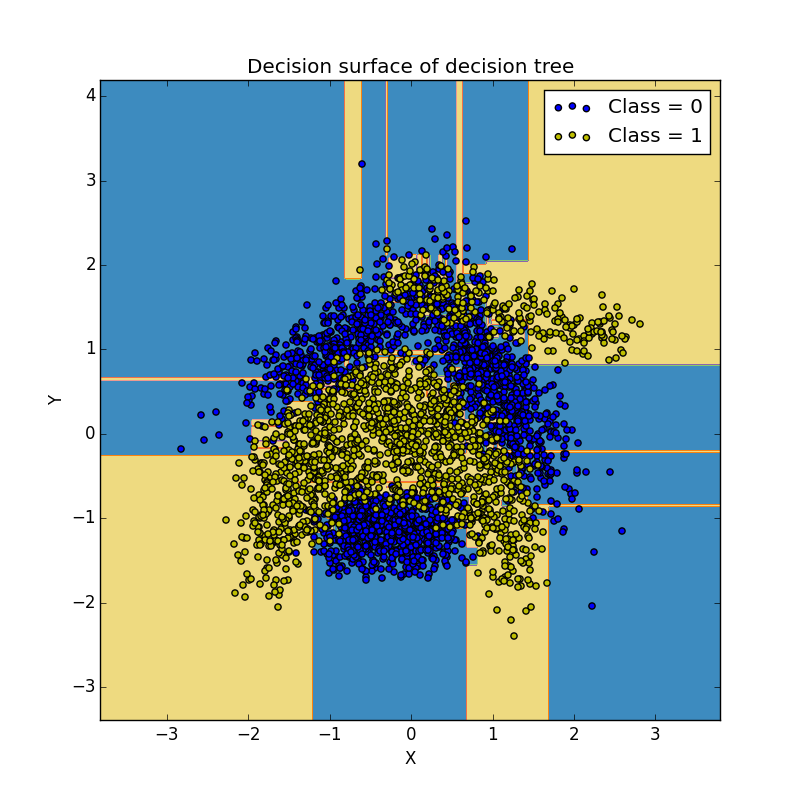
\includegraphics[scale = 0.45]{./../figures/2_1_1.png}
\end{center}
Code to reproduce this plot is included in the appendix.

\subsection*{2.2 Visualizing decision surfaces for trees varying \texttt{max\_depth}}

Next, we grew decision trees varying the hyperparameter \texttt{max\_depth}. Trees were grown for all \texttt{max\_depth}s in $\{1, \cdots, 10\}$; decision surfaces for these trees are shown below.
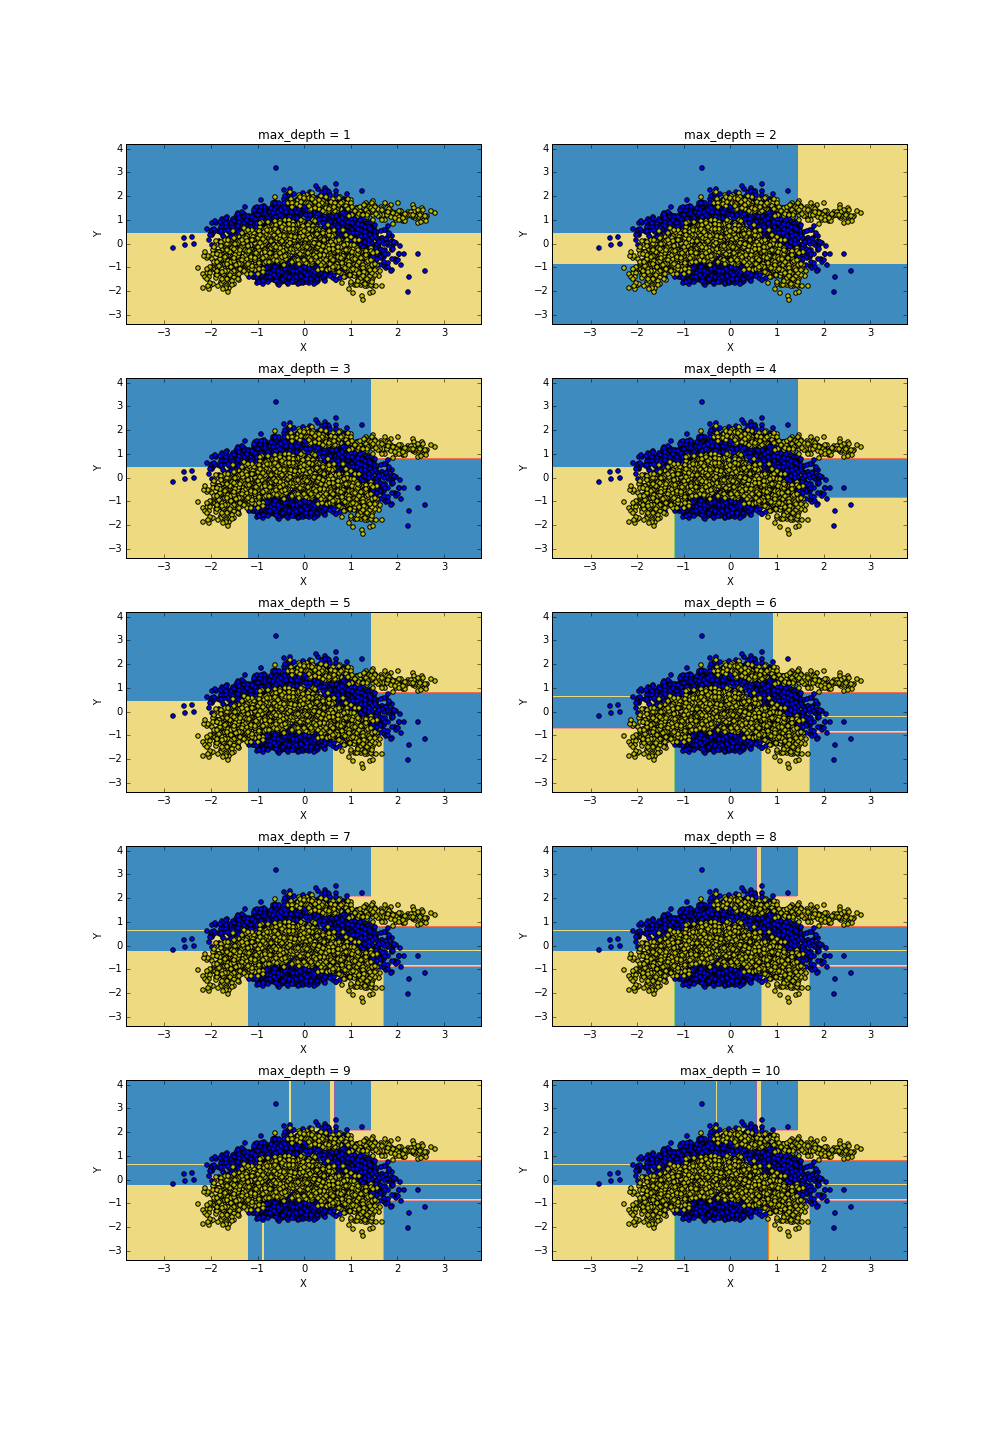
\includegraphics[scale=0.45]{./../figures/2_1_2.png}

From the decision surfaces, it is apparent the complexity of the trees grow with \texttt{max\_depth}. Again, code to reproduce these plots is included in the appendix.

\subsection*{2.3 Comparing train and test errors for varying \texttt{max\_depth}}

Next, we compare the training and test set error rates (average 0-1 loss) for trees of varying \texttt{max\_depth}.
\begin{center}
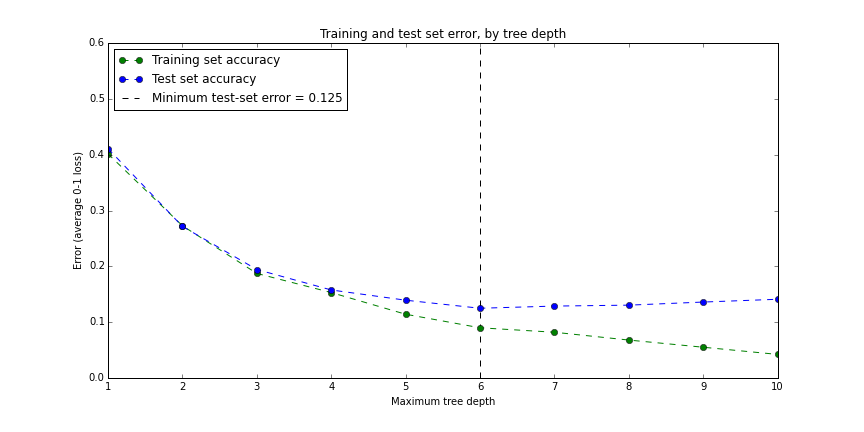
\includegraphics[scale=0.5]{./../figures/2_1_3.png}
\end{center}

The optimal \texttt{max\_depth} is 6, though the test set error curve is relatively flat for \texttt{max\_depth} $\in \{5, \cdots 8\}$. As expected, the training error is strictly decreasing.

\subsection*{2.4 Comparing train and test errors for varying \texttt{max\_depth}}

Using \texttt{scikit-learn}s \texttt{grid\_search.GridSearchCV} function, decision trees were build and compared (using cross-validation performance) for all combinations of
\begin{itemize}
\item \textbf{Criterion}: Gini, entropy
\item \textbf{\texttt{max\_depth}}: 1, 2, 3, 4, 5, 6, 7, 8, 9, 10
\item \textbf{\texttt{min\_samples\_split}}: 2, 4, 8, 16, 32, 64, 128, 256, 512
\item \textbf{\texttt{min\_samples\_leaf}}: 1, 2, 4, 8, 16, 32, 64, 128, 256, 512
\end{itemize}

Based on this grid search, the optimal hyperparameters were found to be
\begin{itemize}
\item \textbf{Criterion}: Gini
\item \textbf{\texttt{max\_depth}}: 9
\item \textbf{\texttt{min\_samples\_split}}: 8
\item \textbf{\texttt{min\_samples\_leaf}}: 2
\end{itemize}

This set of hyperparameters achieved a cross-validation average error rate of 0.8911. However, when this tree was scored using the training set, it only achieved a test-set error rate of 0.137 (which is actually worse than the tree found in 2.1). Hence, we were unable to improve our performance using the hyperparameters tested in our grid search.

%----------------------------------------------------------------------------------------

\section*{3. AdaBoost}
\subsection*{3.1 Implementing AdaBoost}

See the code in the attached appendix.

\subsection*{3.2 Visualizing the AdaBoost training procedure}

AdaBoost was used to fit the Banana dataset, using decision trees of depth 3 as the base classifiers. The algorithm was run for different numbers of rounds $1, \cdots, 10$, and decision boundaries are shown in the following figure. The size of the markers indicates the final sample weights (though, unfortunately, the tail of the weight distribution is too fat to allow for effective visualization of a small number of influential points).

From these plots, we can make a number of (fairly trivial) observations:

\begin{itemize}
\item It is apparent from the shape of the decision surface in the rounds = 1 plot that the base classifier is a tree of depth 3. Note this isn't surprising (since we set this base classifier hyperparameter ourselves)- I was just somewhat surprised since (having forgotten that we set \texttt{max\_depth} to 3 I had the mistaken assumption most tree boosting algorithms use decision stumps.
\item It is apparent the decision surface becomes more complex as we increase the number of rounds. Perhaps more interestingly, modifications to the decision boundary appear to become increasingly marginal (i.e. compare the change from 2 to 3 rounds, to the change from 9 to 10 rounds).
\item Again trivial, but worth noting- the decision boundary is decidedly non-linear. This is obvious from the algorithm (since we're using a linear combination of non-linear functions), but worth noting. If we fit a linear model to this data (using only the two features given, without any additional feature engineering or kernelization) we'd do terribly.
\end{itemize}

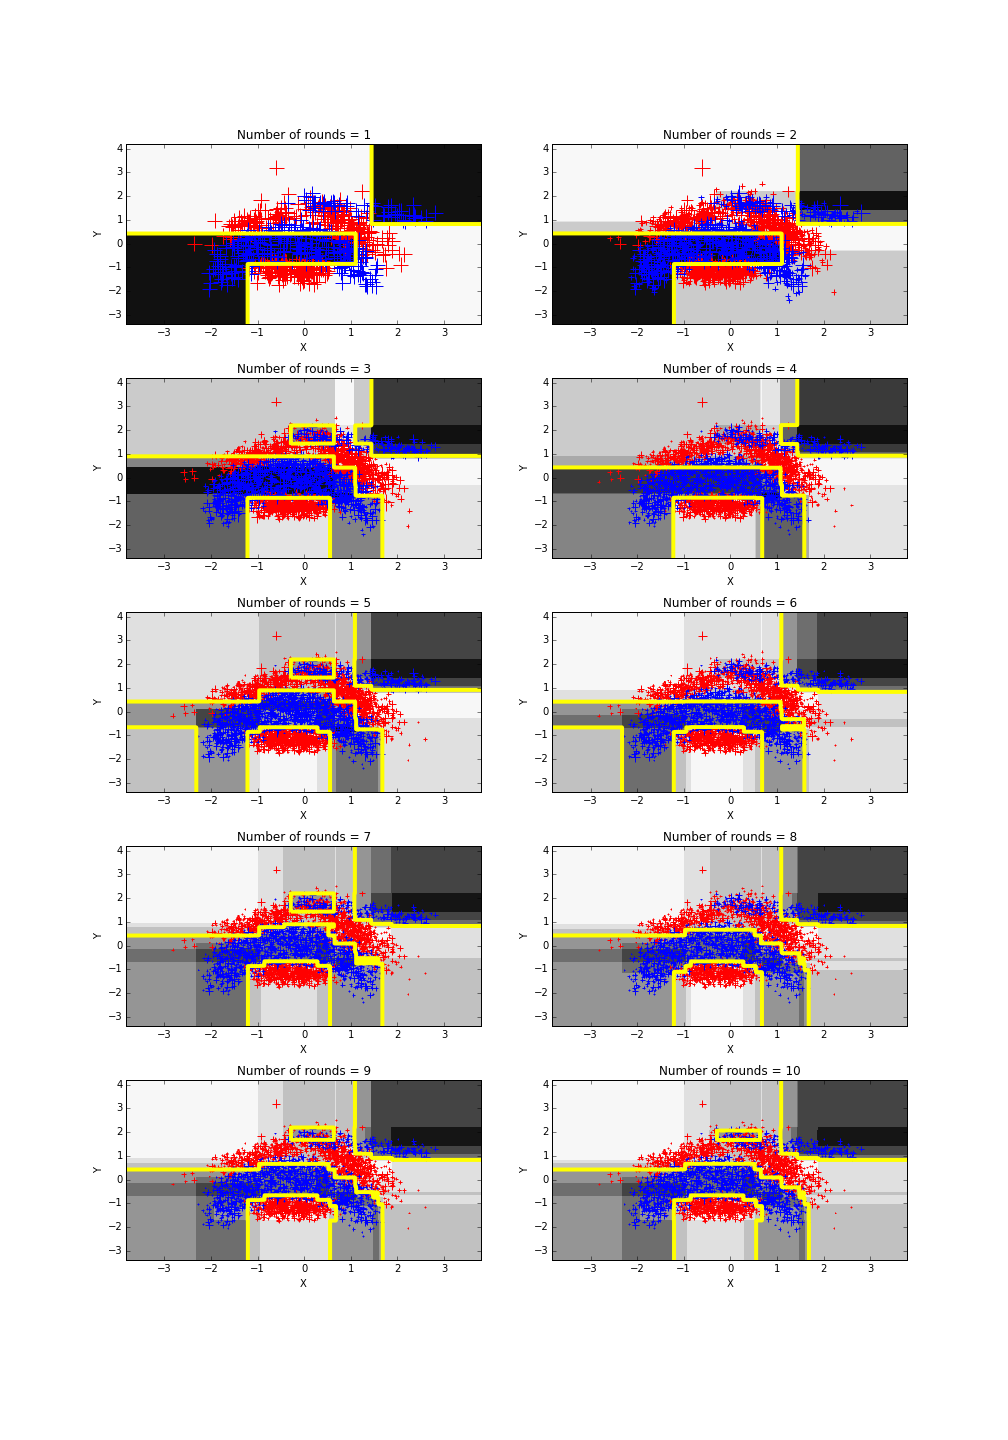
\includegraphics[scale=0.45]{./../figures/3_1_2.png}

\subsection*{3.3 Comparing train and test errors for varying number of rounds}

Next, we compare the training and test set error rates (average 0-1 loss) for AdaBoost with varying numbers of rounds.
\begin{center}
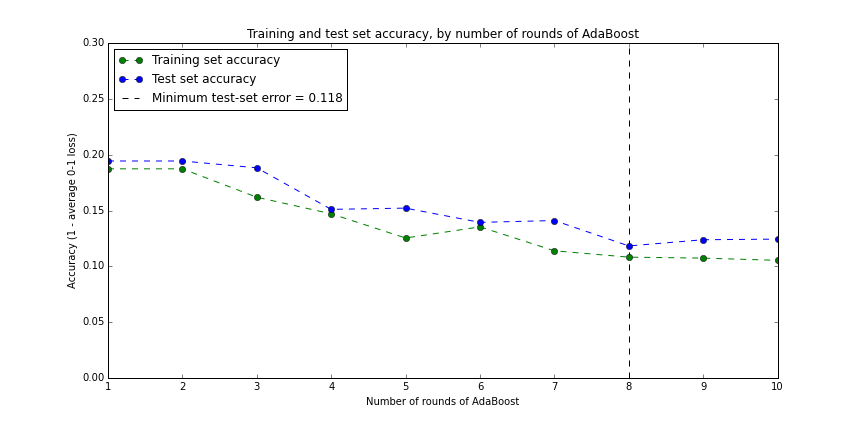
\includegraphics[scale=0.5]{./../figures/3_1_3.png}
\end{center}

The minimum test set error is 0.118, for 8 rounds of AdaBoost (though it essentially appear that after 8 rounds, the test set error has leveled out). The training error is still decreasing (as anticipated) after 10 rounds.

%----------------------------------------------------------------------------------------

\section*{4. Gradient Boosting Machines}
\subsection*{4.1 Basis functions in $L_2$-Boosting}

In this problem, take $\mathcal{Y} = \mathbb{R}$, and suppose our loss function is given by
\[\ell(\hat{y},y) = \frac{1}{2}(\hat{y} - y)^2\]
In the beginning of the $m^{th}$ round of gradient boosting, we have the function $f_{m-1}(x)$.

Our goal is to show the $h_m$ chosen as the next basis function is given by
\[h_m = \arg \min_{h \in \mathcal{F}} \sum_{i = 1}^n [(y_i - f_{m-1}(x_i)) - h(x_i)]^2\]

First, given $f_{m-1}(x)$, the gradient boosting algorithm proceeds by computing $\mathbf{g}_m$.
\begin{align*}
\mathbf{g}_m &= \left( \frac{\partial}{\partial f(x_i)} \sum_{i = 1}^n \ell(y_i, f(x_i)) \Bigg|_{f(x_i) = f_{m - 1}(x_i)} \right)_{i = 1}^n \\
	&= \left( \frac{\partial}{\partial f_{m-1}(x_i)} \sum_{i = 1}^n \ell(y_i, f_{m-1}(x_i)) \right)_{i = 1}^n \\
	&= \left( \frac{\partial}{\partial f_{m-1}(x_i)} \sum_{i = 1}^n \left[\frac{1}{2}(f_{m-1}(x_i) - y_i)^2\right] \right)_{i = 1}^n \\
	&= \left(f_{m-1}(x_i) - y_i\right)_{i = 1}^n \\
\end{align*}

Interestingly (as remarked elsewhere- either a reference text or lecture), $\mathbf{g}_m$ is just the residual vector $r_{m-1}$.

Now we proceed to fit a regression model to $-\mathbf{g}_m$.
\begin{align*}
h_m &= \arg \min_{h \in \mathcal{F}} \sum_{i = 1}^n [(-\mathbf{g}_m)_i - h(x_i)]^2 \\
	&= \arg \min_{h \in \mathcal{F}} \sum_{i = 1}^n [\left(-(f_{m-1}(x_i) - y_i)\right) - h(x_i)]^2 \\
	&= \arg \min_{h \in \mathcal{F}} \sum_{i = 1}^n [(y_i - f_{m-1}(x_i)) - h(x_i)]^2
\end{align*}

which is what we set out to show.

\subsection*{4.2 Basis functions in BinomialBoost (classification with logistic loss)}

Now take $\mathcal{Y} = \{-1, 1\}$, and $\ell(m) = \ln(1 + e^{-m}$, where $m = yf(x)$.

Again, we consider the $m^{th}$ step in gradient boosting, starting with $f_{m-1}(x)$. We again begin by finding $\mathbf{g}_m$.

\begin{align*}
\mathbf{g}_m &= \left( \frac{\partial}{\partial f(x_i)} \sum_{i = 1}^n \ell(y_i, f(x_i)) \Bigg|_{f(x_i) = f_{m - 1}(x_i)} \right)_{i = 1}^n \\
	&= \left( \frac{\partial}{\partial f_{m-1}(x_i)} \sum_{i = 1}^n \ell(y_i, f_{m-1}(x_i)) \right)_{i = 1}^n \\
	&= \left( \frac{\partial}{\partial f_{m-1}(x_i)} \sum_{i = 1}^n \left[\ln (1 + e^{y_i f_{m-1}(x_i)})\right] \right)_{i = 1}^n \\
	&= \left(\frac{-y_i}{1+e^{y_i f_{m-1}(x_i)}}\right)_{i = 1}^n \\
\end{align*}

Finally, we proceed to fit a regression model to $-\mathbf{g}_m$.
\begin{align*}
h_m &= \arg \min_{h \in \mathcal{F}} \sum_{i = 1}^n [(-\mathbf{g}_m)_i - h(x_i)]^2 \\
	&= \arg \min_{h \in \mathcal{F}} \sum_{i = 1}^n \left[\left(- \left(\frac{-y_i}{1+e^{y_i f_{m-1}(x_i)}}\right)\right) - h(x_i)\right]^2 \\
	&= \arg \min_{h \in \mathcal{F}} \sum_{i = 1}^n \left[ \frac{-y_i}{1+e^{y_i f_{m-1}(x_i)}} - h(x_i)\right]^2
\end{align*}

So our expression for $h_m$ is 
\[h_m = \arg \min_{h \in \mathcal{F}} \sum_{i = 1}^n \left[ \frac{-y_i}{1+e^{y_i f_{m-1}(x_i)}} - h(x_i)\right]^2\]

%----------------------------------------------------------------------------------------

\section*{5. From Margins to Conditional Probabilities}
\subsection*{5.1 Expressing $\mathbb{E}_y[\ell(yf(x)) | x]$ in terms of $\pi(x)$ and $\ell(f(x))$}

Let $\pi(x) = P(y = 1 | x)$. Then note (with $y \in \{1, -1\}$
\[(1- \pi(x) = (1 - P(y = 1 | x) = P(y = -1 | x)\]

Now consider $\mathbb{E}_y[\ell(yf(x)) | x]$. Well,
\begin{align*}
\mathbb{E}_y[\ell(yf(x)) | x]  &= \sum_{y \in \{-1, 1\}} \ell(yf(x))P_{Y | X} (y | x) \\
	&= \ell(1\cdot f(x))P(Y = 1 | x) + \ell(-1 \cdot f(x)) P(Y = -1 | x) \\
	&= \ell(f(x))\pi(x) + \ell(-f(x)) (1- \pi(x))	
\end{align*}

\subsection*{5.2 Bayes prediction function for exponential loss function}

Now, let $\ell(y, f(x)) = e^{-y f(x)}$. This is a margin loss, with $m = yf(x)$, so we have $\ell(m) = e^{-m}$.

Now let's find $f^*(x)$. We proceed by differentiating our expression for $\mathbb{E}_y[\ell(yf(x)) | x]$ with respect to $f(x)$:

\begin{align*}
\frac{\partial}{\partial f(x)} \mathbb{E}_y[\ell(yf(x)) | x]  &= \frac{\partial}{\partial f(x)} \left[\ell(f(x))\pi(x) + \ell(-f(x)) (1- \pi(x))	\right] \\
	&= \ell'(f(x))f'(x)\pi(x) - \ell'(-f(x))f'(x)(1- \pi(x))
\end{align*}

Setting this expression equal to zero, and dividing by $f'(x)$ yields
\[\ell'(f(x))\pi(x) - \ell'(-f(x))(1- \pi(x)) = 0 \]
Note $\ell'(m) = - e^{-m}$. Thus, we have
\begin{align*}
-e^{-f(x)} \pi(x) + e^{f(x)}(1 - \pi(x)) &= 0 \\
\implies \qquad{} e^{f(x)}\left(- e^{-f(x)} \pi(x) + e^{f(x)}(1 - \pi(x))\right) &= e^{f(x)} 0 \\
\implies \qquad{} -1 \cdot \pi(x) + e^{2f(x)}(1 - \pi(x)) &= 0 \\
\implies \qquad{} f(x) &= \frac{1}{2} \ln \left(\frac{\pi(x)}{1 - \pi(x)}\right)
\end{align*}

So $f^*(x) = \frac{1}{2} \ln \left(\frac{\pi(x)}{1 - \pi(x)}\right)$.\\

Next, given $f^*(x)$, note
\begin{align*}
f^*(x) &= \frac{1}{2} \ln \left(\frac{\pi(x)}{1 - \pi(x)}\right) \\
\implies \qquad{} 2f^*(x) &= \ln \left(\frac{\pi(x)}{1 - \pi(x)}\right) \\
\implies \qquad{} e^{2f^*(x)} &= \frac{\pi(x)}{1 - \pi(x)} \\
\implies \qquad{} e^{-2f^*(x)} &= \frac{1 - \pi(x)}{\pi(x)} \\
\implies \qquad{} e^{-2f^*(x)} &= \frac{1}{\pi(x)} - 1\\
\implies \qquad{} 1 + e^{-2f^*(x)} &= \frac{1}{\pi(x)} \\
\implies \qquad{} \frac{1}{1 + e^{-2f^*(x)}} &= \pi(x) \\
\end{align*}

\subsection*{5.3 Bayes prediction function for logistic loss function}

Now, let $\ell(y, f(x)) = \ln(1 + e^{-y f(x)})$. Again this is a margin loss (with $m = yf(x)$), so we have
$\ell(m) =  \ln(1 + e^{-m})$. Moreover, $\ell'(m) = \frac{-e^{-m}}{1 + e^{-m}}$.\\

Thus, substituting into $\ell'(f(x))\pi(x) - \ell'(-f(x))(1- \pi(x)) = 0$ yields
\begin{align*}
\frac{-e^{-f(x)}}{1 + e^{-f(x)}}\pi(x) + \frac{e^{f(x)}}{1 + e^{f(x)}}(1- \pi(x)) &= 0 \\
\implies \qquad{} \frac{e^{f(x)}}{1 + e^{f(x)}}(1- \pi(x)) &= \frac{e^{-f(x)}}{1 + e^{-f(x)}}\pi(x)\\
\implies \qquad{} \frac{e^{f(x)}(1 + e^{-f(x)})}{e^{-f(x)}(1 + e^{f(x)})} &= \frac{\pi(x)}{(1- \pi(x))}\\
\implies \qquad{} \frac{e^{f(x)}e^{f(x)}(1 + e^{-f(x)})}{(1 + e^{f(x)})} &= \frac{\pi(x)}{(1- \pi(x))}\\
\implies \qquad{} \frac{e^{f(x)}(e^{f(x)} + 1)}{(1 + e^{f(x)})} &= \frac{\pi(x)}{(1- \pi(x))}\\
\implies \qquad{} e^{f(x)}&= \frac{\pi(x)}{(1- \pi(x))}\\
\implies \qquad{} f(x)&= \ln\left(\frac{\pi(x)}{(1- \pi(x))}\right)\\
\end{align*}

So $f^*(x) =\ln\left(\frac{\pi(x)}{(1- \pi(x))}\right)$.\\

Next, given $f^*(x)$, note
\begin{align*}
f^*(x) &= \ln\left(\frac{\pi(x)}{(1- \pi(x))}\right) \\
\implies \qquad{} e^{f^*(x)} &= \frac{\pi(x)}{(1- \pi(x))} \\
\implies \qquad{} e^{-f^*(x)} &= \frac{(1- \pi(x))}{\pi(x)}\\
\implies \qquad{} e^{-f^*(x)} &= \frac{1}{\pi(x)} - 1\\
\implies \qquad{} 1 + e^{-f^*(x)} &= \frac{1}{\pi(x)}\\
\implies \qquad{} \frac{1}{1 + e^{-f^*(x)}} &= \pi(x)
\end{align*}

\subsection*{5.4 Bayes prediction function for hinge loss function}

Now take $\ell(y, f(x)) = \max\{0, 1 - yf(x)\}$.\\

Again, this is a margin loss, with $\ell(m) = \max\{0, 1 - m\}$. \\

Recall we want to minimize $\ell(f(x))\pi(x) + \ell(-f(x)) (1- \pi(x))$. Since $\ell$ is no longer differentiable (over all $m$), we'll need to use its subdifferential. Our goal is to find $f^*(x)$ that minimizes this expression (i.e. values of $f^*(x)$ where 0 is in the subdifferential).\\

First, note
\[
\partial \left[\ell(f(x))\pi(x) + \ell(-f(x)) (1- \pi(x)) \right] = \partial\ell(f(x)) \partial f(x) \pi(x) - \partial \ell(-f(x)) \partial f(x) (1- \pi(x))\]

Thus, if
 \[
0 \in \partial\ell(f(x)) \partial f(x) \pi(x) - \partial \ell(-f(x)) \partial f(x) (1- \pi(x))
\]
then there exists $g$'s in the $\partial$'s such that
\begin{align*}
g_{\partial \ell(f(x))} g_{\partial f(x)} \pi(x) - g_{\partial \ell(-f(x))} g_{\partial f(x)} (1- \pi(x)) = 0 \\
\implies \qquad{} g_{\partial \ell(f(x))} \pi(x) - g_{\partial \ell(-f(x))} (1- \pi(x)) = 0 
\end{align*}

Now, note
\[
\partial \ell(f(x)) =
\begin{cases}
{0} & \textrm{ for } f(x) > 1 \\
[-1, 0] & \textrm{ for } f(x) = 1 \\
{-1} & \textrm{ for } f(x) < 1 \\
\end{cases}
\]

and 

\[
\partial \ell(-f(x)) =
\begin{cases}
{0} & \textrm{ for } f(x) < -1 \\
[0, 1] & \textrm{ for } f(x) = -1 \\
{1} & \textrm{ for } f(x) > -1 \\
\end{cases}
\]

Thus, substituting we can construct 

\[
\partial \left[\ell(f(x))\pi(x) + \ell(-f(x)) (1- \pi(x)) \right] =
\begin{cases}
(1 - \pi(x)) & \textrm{ for } f(x) > 1 \\
a \pi(x) + (1 - \pi(x)), -1 \leq a \leq 0 & \textrm{ for } f(x) = 1 \\
- \pi(x) + (1 - \pi(x)) & \textrm{ for } -1 < f(x) < 1 \\
- \pi(x) + b (1 - \pi(x)), 0 \leq b \leq 1 & \textrm{ for } f(x) = -1 \\
- \pi(x) & \textrm{ for } f(x) < -1 \\
\end{cases}
\]

This yields our solution:

\begin{itemize}
\item \textbf{Case 1}: If $\pi(x) = 1$, then $f^*(x) = c$ for any $c \geq 1$.
\item \textbf{Case 2}: If $\pi(x) = 0$, then $f^*(x) = c$ for any $c \leq -1$. 
\item \textbf{Case 3}: If $\pi(x) = \frac{1}{2}$, then $f^*(x) = c$ for any $-1 \leq c \leq 1$. 
\item \textbf{Case 4}: If $\pi(x) < \frac{1}{2}$, then $f^*(x) = -1$. To see that $0 \in \partial$ at $f^*(x) = -1$, take $b = \frac{\pi(x)}{1 - \pi(x)}$ (which is clearly in $[0,1]$). Then \\
$-\pi(x) + b(1 - \pi(x))  = -\pi(x) + \frac{\pi(x)}{1 - \pi(x)}(1 - \pi(x)) = -\pi(x) + \pi(x) = 0$
\item \textbf{Case 5}: If $\pi(x) > \frac{1}{2}$, then $f^*(x) = 1$. To see  $0 \in \partial$ at $f^*(x) = 1$, take $a = \frac{\pi(x) - 1}{\pi(x)}$ (which is clearly in $[-1,0]$). Then \\
$a \pi(x) + (1 - \pi(x))  = \frac{\pi(x) - 1}{\pi(x)} \pi(x) + (1 - \pi(x)) =\pi(x) - 1 + (1 - \pi(x)) = 0$
\end{itemize}

We can summarize these cases quite simply by stating:
\[f^*(x) = \textrm{sign}\left(\pi(x) - \frac{1}{2}\right)\] 


%----------------------------------------------------------------------------------------

\section*{6. AdaBoost Actually Works- Exponential Bound on Training Loss}

Our objective in this section is to place an exponential bound on the AdaBoost training loss. We do so by proving a number of inequalities, then putting them together in subsection 6.

\subsection*{6.1 $1(g(x) \ne y) < \exp(-yg(x))$}

We start be showing for any function $g$ into \{-1, +1\}, $1(g(x) \ne y) < \exp(-yg(x))$. We show this explicitly (through enumeration):
\begin{center}
\begin{tabular}{ | c | c | c | c |}
\hline
$g(x)$ & $y$ & $1(g(x) \ne y)$ & $\exp(-y g(x))$ \\
\hline
-1 & -1 & 0 & $\exp(-(-1)(-1)) = e^{-1}$ \\
\hline
-1 & 1 & 1& $\exp(-(-1)(1)) = e$ \\
\hline
1 & -1 & 1 & $\exp(-(1)(-1)) = e$ \\
\hline
1 & 1 & 0 & $\exp(-(1)(1)) = e^{-1}$ \\
\hline
\end{tabular}
\end{center}

\subsection*{6.2 $L(G,D) < Z_T$}

Now we show $L(G,D) < Z_T$. First, recall

\[L(G,D) = \frac{1}{n} \sum_{i=1}^n 1(G(x_i) \ne y_i)\]

Now let's consider two cases:
\begin{itemize}
\item For $i$ such that $G(x_i) \ne y_i$, we have
\[1(G(x_i) \ne y_i) = 1\]
while
\[\exp(-y_i f_T(x_i)) = \exp(-y_i \sum_{t = 1}^T \alpha_t G_t(x_i))\]
By $G(x_i) \ne y_i$, the definition of $G$ implies $-y_i \sum_{t = 1}^T \alpha_tG_t(x_i) \geq 0$, so 
\[\exp(-y_i f_T(x_i)) \geq 1 = 1(G(x_i) \ne y_i)\]
\item For $i$ such that $G(x_i) = y_i$, we have
\[1(G(x_i) \ne y_i) = 0\]
while $\exp(-y_i f_T(x_i)) > 0 $, so 
\[\exp(-y_i f_T(x_i)) > 0 = 1(G(x_i) \ne y_i)\]
Thus, matching term by term yields 

\[L(G,D) = \frac{1}{n} \sum_{i=1}^n 1(G(x_i) \ne y_i) < \frac{1}{n} \sum_{i=1}^n \exp(-y_i f_T(x_i)) = Z_T \]
\end{itemize}

\subsection*{6.3 $w_i^{t+1} < \exp(-y_i f_t(x_i))$}

We take a slightly modified approach here, and show $w_i^{t+1} < \frac{1}{n} \exp(-y_i f_t(x_i))$ using induction:

Base case: Let  $t = 1$. Then (recalling $w_i^1 = \frac{1}{n}$)
\begin{align*}
w_i^{t+1} = w_i^2 &= w_i^1 e^{(-\alpha_1 y_i G_1(x_i))} \\
=& \frac{1}{n} e^{(-y_i f_1(x_i))} \\
=& \frac{1}{n} e^{(-y_i f_t(x_i))}
\end{align*}

Now assume $w_i^t = \frac{1}{n} e^{(-y_i f_{t-1}(x_i))}$. Then

\begin{align*}
w_i^{t+1} &= w_i^t e^{(-\alpha_t y_i G_t(x_i))} \\
&= \frac{1}{n} e^{(-y_i f_{t-1}(x_i))} e^{(-\alpha_t y_i G_t(x_i))} \\
&= \frac{1}{n} e^{(-y_i [ f_{t-1}(x_i)+\alpha_t G_t(x_i)])} \\
&= \frac{1}{n} e^{(-y_i f_{t}(x_i))}
\end{align*}

\subsection*{6.4 $\frac{Z_{t+1}}{Z_t} = 2 \sqrt{\mathrm{err}_{t+1}(1 - \mathrm{err}_{t+1})}$}

Starting from $\frac{Z_{t+1}}{Z_t}$, we find

\begin{align*}
\frac{Z_{t+1}}{Z_t} &= \frac{1/n \sum_{i =1}^n \exp(-y_i f_{t+1}(x_i))}{1/n \sum_{i =1}^n \exp(-y_i f_{t}(x_i))} \\
&= \frac{\sum_{i =1}^n 1/n \exp(-y_i f_{t+1}(x_i))}{ \sum_{i =1}^n 1/n \exp(-y_i f_{t}(x_i))} \\
&= \frac{\sum_{i =1}^n w_i^{t+2}}{ \sum_{i =1}^n w_i^{t+1}} \\
&= \frac{\sum_{i =1}^n w_i^{t+1}\exp(-\alpha_{t+1}y_iG_t(x_i))}{ \sum_{i =1}^n w_i^{t+1}}
\end{align*}
Now we split the sum in the numerator into two sums: first, over $i$ such that $y_i = G_t(x_i)$ (so $y_i G_t(x_i) = 1$), and second, over $i$ such that $y_i \ne G_t(x_i)$ (so $y_i G_t(x_i) = -1$). 

\begin{align*}
\frac{Z_{t+1}}{Z_t} &=\frac{\sum_{i =1}^n w_i^{t+1}\exp(-\alpha_{t+1}y_iG_t(x_i))}{ \sum_{i =1}^n w_i^{t+1}} \\
&= \frac{\sum_{i =1}^n w_i^{t+1} 1(G_t(x_i) \ne y_i) \exp(\alpha_{t+1})}{ \sum_{i =1}^n w_i^{t+1}}  +  \frac{\sum_{i =1}^n w_i^{t+1} 1(G_t(x_i) = y_i) \exp(-\alpha_{t+1})}{ \sum_{i =1}^n w_i^{t+1}} \\
&= \mathrm{err}_{t+1}\exp(\alpha_{t+1}) + (1- \mathrm{err}_{t+1})\exp(-\alpha_{t+1}) \\
&= \mathrm{err}_{t+1}\exp(1/2 \log(1/ \mathrm{err}_{t+1} - 1)) + (1- \mathrm{err}_{t+1})\exp(-1/2 \log(1/ \mathrm{err}_{t+1} - 1)) \\
&= \mathrm{err}_{t+1}(1/ \mathrm{err}_{t+1} - 1)^{1/2} + (1- \mathrm{err}_{t+1})(1/ \mathrm{err}_{t+1} - 1)^{-1/2} \\
&= (\mathrm{err}_{t+1}^2(1/ \mathrm{err}_{t+1} - 1))^{1/2} + \mathrm{err}_{t+1}(1/\mathrm{err}_{t+1} - 1)(1/ \mathrm{err}_{t+1} - 1)^{-1/2} \\
&= (\mathrm{err}_{t+1}^2(1/ \mathrm{err}_{t+1} - 1))^{1/2} + (\mathrm{err}_{t+1}^2(1/ \mathrm{err}_{t+1} - 1))^{1/2}\\
&= 2\sqrt{(\mathrm{err}_{t+1}(1 - \mathrm{err}_{t+1})}
\end{align*}

\subsection*{6.5 Showing $\frac{Z_{t+1}}{Z_t} \leq \exp(-2 \gamma^2)$}

We show this statement is true in three steps. First, we show the function $g(a) = a(1-a)$ is monotonically increasing on [0,1/2]. Then we show that $1-a \leq \exp(-a)$. Finally, we put it together to get the desired result.

First, consider $g(a) = a(1-a)$. Then note $g'(a) = 1-2a \geq 0$ for all $a \in [0,1/2]$. Thus $g$ is monotonically increasing over the interval [0,1/2].

Next, consider $1-a \leq \exp(-a)$. Note the second derivative of $\exp(-a)$ is $\exp(-a) > 0$ for all $a$. Thus, this is a convex function. As such, it lies above its tangent at all points- in particular it lies above it's tangent at 0, so:
\begin{align*}
\exp(-a) &\geq \exp(-0) + (-\exp(-0))(a - 0) \\
\exp(-a) &\geq 1 + (-1)(a) \\
\exp(-a) &\geq 1 - a
\end{align*}

Finally, we tackle the expression $\frac{Z_{t+1}}{Z_t}$. 

First, if $\textrm{err}_{t+1} < 1/2 - \gamma \leq 1/2$, then (using our earlier result that $g(a)$ is monotonically increasing for $a \in [0,1/2]$)
\begin{align*}
(\textrm{err}_{t+1}) (1 - \textrm{err}_{t+1}) &\leq (1/2 - \gamma)(1 - (1/2 - \gamma)) \\
&\leq (1/2 - \gamma)(1/2 + \gamma)) \\
&\leq 1/4  - \gamma^2 \\
&\leq 1/4 ( 1 - 4 \gamma^2)
\end{align*}

Then, (by our lower bound on $\exp(-a)$) we also have
\[(\textrm{err}_{t+1}) (1 - \textrm{err}_{t+1}) \leq 1/4 ( 1 - 4 \gamma^2) \leq 1/4 \exp(-4 \gamma^2) \]

So substituting yields
\begin{align*}
\frac{Z_{t+1}}{Z_t} &= 2 \sqrt{(\textrm{err}_{t+1}) (1 - \textrm{err}_{t+1})} \\
&\leq 2 \sqrt{1/4 \exp(-4 \gamma^2)} \\
&\leq 2 \cdot1/2 \sqrt{\exp(-2 \gamma^2)^2} \\
&\leq \exp(-2 \gamma^2)
\end{align*}

\subsection*{6.6 Completing proof}

By 2, we have $L(G, D) < Z_T$. Thus,
\begin{align*}
L(G, D) &< Z_T \\
L(G, D) &< \frac{Z_T}{Z_{T-1}} \cdot  \frac{Z_T-1}{Z_{T-2}} \cdots  \frac{Z_2}{Z_{1}} \cdot \frac{Z_1}{Z_{0}} \cdot Z_0 \\
&\leq \exp(-2 \gamma^2)^{T} Z_0  \\
&\leq \exp(-2 T \gamma^2)^{}
\end{align*}

Note, to complete this proof, we assume we start with a round 0, where $f \equiv 0$, so $Z_0 = 1$.

%----------------------------------------------------------------------------------------

\section*{7. AdaBoost is FSAM with Exponential Loss}

Our objective in this section is to show AdaBoost is FSAM with exponential loss. 

\subsection*{7.1 Write first step of additive model with exponential loss}

Recall the exponential loss function is $L(y, f(x)) = \exp(-y, f(y))$.

The first step in the additive model is to compute
\[
(\alpha_t, G_t) = \arg \min_{\alpha, G} \sum_{i = 1}^n L(y_i, f_{t-1}(x_i) + \alpha G(x_i))\]

Substituting in the exponential loss function yields
\begin{align*}
(\alpha_t, G_t) &= \arg \min_{\alpha, G} \sum_{i = 1}^n L(y_i, f_{t-1}(x_i) + \alpha G(x_i))\\
&= \arg \min_{\alpha, G} \sum_{i = 1}^n \exp(-y_i (f_{t-1}(x_i) + \alpha G(x_i)))\\
&= \arg \min_{\alpha, G} \sum_{i = 1}^n \left[ \exp(-y_i f_{t-1}(x_i)) \exp(-y_i \alpha G(x_i))) \right]
\end{align*}
Now, from question 6, we know to set $w_i^{t} = 1/n \exp(-y_i f_{t-1}(x_i))$, so substitution yields
\[(\alpha_t, G_t) = \arg \min_{\alpha, G} \sum_{i = 1}^n \left[n w_i^t \exp(-y_i \alpha G(x_i))\right] = \arg \min_{\alpha, G} \sum_{i = 1}^n \left[w_i^t \exp(-y_i \alpha G(x_i))\right] \]

\subsection*{7.2 Solving for $G_t$ for a fixed positive $\alpha$}

Now consider $\alpha$ fixed. We want to find
\[ G_t = \arg \min_{G} \sum_{i = 1}^n \left[w_i^t \exp(-y_i \alpha G(x_i))\right] \]

We proceed by splitting the sum in part 1 into two parts:  first, over $i$ such that $y_i = G(x_i)$ (so $y_i G(x_i) = 1$), and second, over $i$ such that $y_i \ne G(x_i)$ (so $y_i G(x_i) = -1$). Then

\[ G_t = \arg \min_{G} \sum_{i = 1}^n \left[w_i^t \exp(-\alpha) 1(G(x_i) = y_i)\right] + \sum_{i = 1}^n \left[w_i^t \exp(\alpha) 1(G(x_i) \ne y_i)\right] \]

Now consider any particular $x_i$: note either $G(x_i) = y_i$ or $G(x_i) \ne y_i$ (since every $G$ in AdaBoost maps $x_i 
\mapsto \{1, -1\}$). In addition, note (for any $\alpha > 0$)
\[w_i^t \exp(-\alpha) < w_i^t \exp(\alpha)\]

Thus, $G_t$ that minimizes $\sum_{i = 1}^n \left[w_i^t 1(G(x_i) \ne y_i)\right]$ also minimizes our objective, so

\[ G_t = \arg \min_{G} \sum_{i = 1}^n \left[w_i^t 1(G(x_i) \ne y_i)\right] \]

\subsection*{7.3 Solving for $\alpha_t$}

Now we plug this $G_t$ back into the first equation and solve for $\alpha$.
\begin{align*}
 \sum_{i = 1}^n \left[w_i^t \exp(-y_i \alpha G(x_i))\right] & = 
 \sum_{i = 1}^n \left[w_i^t \exp(-\alpha) 1(G_t(x_i) = y_i)\right] + \sum_{i = 1}^n \left[w_i^t \exp(\alpha) 1(G_t(x_i) \ne y_i)\right] \\
 & =\exp(-\alpha) \sum_{i = 1}^n \left[w_i^t 1(G_t(x_i) = y_i)\right] + \exp(\alpha)  \sum_{i = 1}^n \left[w_i^t 1(G_t(x_i) \ne y_i)\right] \\
\end{align*}

Now let's get notation under control. Let
\begin{align*}
c_= &=  \sum_{i = 1}^n \left[w_i^t 1(G_t(x_i) = y_i)\right] \\
c_{\ne} &= \sum_{i = 1}^n \left[w_i^t 1(G_t(x_i) \ne y_i)\right]
\end{align*}
Note, as well, that
\[c_= + c_{\ne} = \sum_{i = 1}^n \left[w_i^t 1(G_t(x_i) = y_i)\right] + \sum_{i = 1}^n \left[w_i^t 1(G_t(x_i) \ne y_i)\right] = \sum_{i = 1}^n w_i^t\]

Now let's substitute:
\begin{align*}
 \sum_{i = 1}^n \left[w_i^t \exp(-y_i \alpha G(x_i))\right]
 & =\exp(-\alpha) \sum_{i = 1}^n \left[w_i^t 1(G_t(x_i) = y_i)\right] + \exp(\alpha)  \sum_{i = 1}^n \left[w_i^t 1(G_t(x_i) \ne y_i)\right] \\
& = \exp(-\alpha) c_= + \exp(\alpha) c_{\ne}
\end{align*}

To minimize with respect to $\alpha$, we take the derivative and set it to 0:
\begin{align*}
\frac{\textrm{d}}{\textrm{d}\alpha} [\exp(-\alpha) c_= + \exp(\alpha) c_{\ne}] = -\exp(-\alpha) c_= + \exp(\alpha) c_{\ne} &\triangleq 0 \\
\implies \qquad{} \exp(2\alpha)c_{\ne} &= c_= \\
\implies \qquad{} \exp(2\alpha) &= \frac{c_=}{c_{\ne}} \\
\implies \qquad{} \alpha &= \frac{1}{2} \log \frac{c_=}{c_{\ne}} \\
\implies \qquad{} \alpha &= \frac{1}{2} \log \left( \frac{c_= + c_{\ne}}{c_{\ne}} - 1 \right) \\
\implies \qquad{} \alpha &= \frac{1}{2} \log \left(\frac{\sum_{i = 1}^n w_i^t}{\sum_{i = 1}^n \left[w_i^t 1(G_t(x_i) \ne y_i)\right] }- 1 \right) \\
\implies \qquad{} \alpha &= \frac{1}{2} \log \left(\frac{1}{\textrm{err}_{t}} - 1 \right) \\
\end{align*}

So, we've now shown:
\[\alpha_t = \frac{1}{2} \log \left(\frac{1}{\textrm{err}_{t}} - 1 \right)\]

\subsection*{7.4 Finding weight iterations}

First, recall that $w_i^{t} = 1/n \exp(-y_i f_{t-1}(x_i))$.

Then note
\begin{align*}
w_i^{t+1} &= 1/n \exp(-y_i f_{t}(x_i)) \\
&= 1/n \exp(-y_i \left[f_{t-1}(x_i) + \alpha_t G_t(x_i)\right]) \\
&= 1/n \exp(-y_i f_{t-1}(x_i))\exp(-y_i \alpha_t G_t(x_i)) \\
&= w_i^{t} \exp(-y_i \alpha_t G_t(x_i))
\end{align*}

Thus, we've shown AdaBoost is equivalent to FSAM with exponential loss.

%----------------------------------------------------------------------------------------

\end{document}